\chapter{OpenCAL}

With the name OpenCAL, we identify the sequential version of the
software library, which runs on just a single core of your CPU. It
represents the basis for the other parallel versions. Moreover, it
allows for some \emph{unsafe operations}, which can significantly speed up
your application. Such unsafe operation can also be found in the
OpenMP version, while they are not present to GPU one.

In the following sections, we will introduce OpenCAL by examples. In
the first part of the Chapter, we will deal with the OpenCAL's safe
mode, while in the last one, we will go deep inside OpenCAL,
discussing unsafe operations.

\section{Conway's Game of Life}

In order to introduce you to Cellular Automata development with
OpenCAL, we start this section by implementing the Conway's Game of
Life. It represents one of the most simple, yet powerful examples of
Cellular Automata, devised by the mathematician John Horton Conway in
1970.

The Game of Life can be thought as an infinite two-dimensional
orthogonal grid of square cells (the cellular space), each of which is
in one of two possible states, dead or alive. Every cell interacts
with its eight neighbors, which are the cells that are directly
horizontally, vertically, or diagonally adjacent to it (the Moore
neighborhood). At each time step, one of the following transitions
occur:

\begin{enumerate}
    \item Any live cell with fewer than two alive neighbors dies, as
      if by loneliness.
    \item Any live cell with more than three alive neighbors dies, as
      if by overcrowding.
    \item Any live cell with two or three alive neighbors lives,
      unchanged, to the next generation.
    \item Any dead cell with exactly three live neighbors comes to
      life.
\end{enumerate}

The initial configuration of the system specifies the state (dead or
alive) of each cell into the cellular space. The evolution of the
system is thus obtained by applying the above rules (the CA transition
function) simultaneously to every cell in the cellular space, so that
each new configuration is function of the one at the previous
step. The rules continue to be applied repeatedly to create further
generations. For more details on the Game of life you can check
Wikipedia at the URL
\url{http://en.wikipedia.org/wiki/Conway's_Game_of_Life}.

The program below shows a simple Game of Life sequential
implementation in C with OpenCAL.

\lstinputlisting[float,floatplacement=H, label=lst:cal_life, caption=An OpenCAL implementation of the Conway's game of Life.]{../opencal/OpenCAL/examples/cal_life/source/life.c}

As you can see, even if Listing \ref{lst:cal_life} is very short, it
completely defines the Conway's Game of Life CA and perform a
simulation (actually, only one step in this example). In order to use
OpenCAL, you need to include some header files (lines
3-5). Specifically, among other things, \verb'cal2D.h' (line 3) allows
you to define the CA object (line 9) and the related substate (line
10), while \verb'cal2DRun.h' (line 5) allows you to define a CA
simulation object (line 11), needed to run the CA model. The
\verb'cal2DIO.h' header file (line 4) provides you some input/output
functions for reading/writing substates from/to file.

While statements at lines 9-11 just declare the required objects, they are
defined later in the \verb'main' function. In particular, the life CA
object is defined at line 29 by the \verb'calCADef2D()' function. The
first 2 parameters define the CA dimensions (the number of rows and
columns, respectively), while the third the neighbourhood pattern. The
fourth parameter specifies the boundary conditions. In this case, the CA
cellular space is considered as a torus, with cyclic behaviour at
boundaries. The last parameter allows you to specify if your model
has to use the so called \emph{active cells optimization}, that is
able to restrict the computation to only \emph{non-stationary cells}. In this
case, no optimization is considered.  The complete definition of
\verb'calCADef2D()' is provided in Listing \ref{lst:calCADef2D}.

\begin{lstlisting}[float,floatplacement=H, label=lst:calCADef2D, caption=Definition of the calCADef2D() function., numbers=none]
  struct CALModel2D* calCADef2D (
    int rows,
    int columns,
    enum CALNeighborhood2D CAL_NEIGHBORHOOD_2D,
    enum CALSpaceBoundaryCondition CAL_TOROIDALITY,
    enum CALOptimization CAL_OPTIMIZATION
  )
\end{lstlisting}  

In particular, the \verb'CALNeighborhood2D' enum type (Listing
\ref{lst:CALNeighborhood2D}) allows you to select one of the square or
hexagonal predefined neighbourhoods, or a custom neighbourhood, whose
pattern can be defined directly in your application. Custom
neighbourhoods will be discussed later in this Chapter. Similarly, the
\verb'CALSpaceBoundaryCondition' enum type (Listing
\ref{lst:CALSpaceBoundaryCondition}) allows you to set non-ciclic or
cyclic behaviour at the boundaries of the cellular space. Eventually,
the \verb'CALOptimization' enum type (Listing
\ref{lst:CALOptimization}) allows you to use or not the active cells
optimization.

\begin{lstlisting}[float,floatplacement=H, label=lst:CALNeighborhood2D, caption=The CALNeighborhood2D enum type., numbers=none]
  enum CALNeighborhood2D { 
    CAL_CUSTOM_NEIGHBORHOOD_2D,
    CAL_VON_NEUMANN_NEIGHBORHOOD_2D,
    CAL_MOORE_NEIGHBORHOOD_2D,
    CAL_HEXAGONAL_NEIGHBORHOOD_2D,
    CAL_HEXAGONAL_NEIGHBORHOOD_ALT_2D 
};
\end{lstlisting}  

\begin{lstlisting}[float,floatplacement=H, label=lst:CALSpaceBoundaryCondition, caption=The CALSpaceBoundaryCondition enum type., numbers=none]
  enum CALSpaceBoundaryCondition{
    CAL_SPACE_FLAT = 0,         
    CAL_SPACE_TOROIDAL
  };
\end{lstlisting}

\begin{lstlisting}[float,floatplacement=H, label=lst:CALOptimization, caption=The CALOptimization enum type., numbers=none]
  enum CALOptimization{
    CAL_NO_OPT = 0,
    CAL_OPT_ACTIVE_CELLS        
  };
\end{lstlisting}

The CA simulation object is defined at line 30 by the
\verb'calRunDef2D()' function. The first parameter is a pointer to a
CA object (\verb'life' in our case), while the second and third parameters
specify the initial and last simulation step, respectively. In this
case, we just perform one step of computation, being both the first
and last step set to 1. The last parameter allows you to specify the
substate update policy. It can be implicit or explicit. In the first
case, OpenCAL does substates' updates for you, while in the second case
the substates' updates is your responsibility. Note that, in case
implicit update policy is applyied, all the CA substates are updated
after the execution of each elementary process composing the CA
transition function. We will discuss update policies later in
this Chapter. The complete definition of \verb'calRunDef2D()' is
provided in Listing \ref{lst:calRunDef2D()}. The \verb'CALUpdateMode'
type (Listing \ref{lst:CALUpdateMode}) enumerates possible update
policies.

\begin{lstlisting}[float,floatplacement=H, label=lst:calRunDef2D(), caption=Definition of the calRunDef2D() function., numbers=none]
  struct CALRun2D* calRunDef2D (
    struct CALModel2D* ca2D,
    int initial_step,
    int final_step,
    enum CALUpdateMode UPDATE_MODE 
  )	
\end{lstlisting}

\begin{lstlisting}[float,floatplacement=H, label=lst:CALUpdateMode, caption=The CALUpdateMode enum type., numbers=none]
  enum CALUpdateMode {
    CAL_UPDATE_EXPLICIT = 0,
    CAL_UPDATE_IMPLICIT
  };
\end{lstlisting}

Line 33 allocates memory and registers the substate \verb'Q' to the
\verb'life' CA, while line 36 adds an elementary process to the cell
transition function. The \verb'calAddSubstate2Di()' function is very
simple and self-explanatory. At the contrary,
\verb'calAddElementaryProcess2D()' must be discussed more in detail. It
takes the handle to the CA model to which the elementary process must
be attached and a pointer to a callback function, that defines the
elementary process itself. In our example, we specified
\verb'life_transition_function' as second parameter, being it the name
of a developer-defined function that you can find at lines 14-24. As
you can see, the elementary process callback returns
\verb'void'. Moreover, it takes a pointer to a CA object as first
parameter, followeb by a couple of integers, representing the
coordinates of the generic cell in the CA space. This is the function
prototype which is common to each elementary process you add to your
application. Note that, each elementary process is applyed by OpenCAL
simultaneously to each cell of the cellular space in a computational
step. However, this is completely transparent to the user, so that he/she
can concentrate his/her effort on the definition of single cell behaviour.

When the user is going to implement an elementary process, by defining
its callback function, he/she can rely on a set of OpenCAL functions that
allow to get the substates values of both the central and the
neighbouring cells, and to update the substates values of the central
cell. In the specific case of the Game of Life, we used the
\verb'calGet2Di()' function to get the central cell's value of the
substate \verb'Q' (remember that the central cell is identified by the
coordinates (i, j), coming from the callback parameters), the
\verb'calGetX2Di()' function to get the value of the n-th neighbour's
substate \verb'Q', and the \verb'calSet2Di()' function to update the
value of the substate \verb'Q' for the central cell. In the Game of
Life example, we defined just one elementary process, that therefore
represents the whole cell transition function. However, as we will see
later, many elementary processes can be defined in OpenCAL by simply
calling the \verb'calAddElementaryProcess2D()' function many times. If
you define more than one elementary process, they will be executed in
the order they are added to the CA.

The \verb'calInitSubstate2Di()' function at line 39 sets the whole
substate \verb'Q' to the value 0, i.e. the value of the substate
\verb'Q' is set to 0 in each cell of the cellular space. The following
lines, from 42 to 46, set the value of the substate \verb'Q' for some
cells to 1, in order to define a well known \emph{glider} pattern. In
this case, we provided the cells coordinates as the third and fourth
parameters. In this way, we define the initial condition of the system
direcly inside the \verb'main' function. However, as we will see later
in this Chapter, such kind of initialization can be performed by means
of a specific function.

The \verb'calSaveSubstate2Di()' function (line 49) saves the substate
\verb'Q' to file, while the \verb'calRun2D()' function (line 52)
enters the simulation loop (actually, only one computational step in
this example), and returns to the \verb'main' function when the
simulation is complete. The \verb'calSaveSubstate2Di()' is thus called
again at line 55 to save the new (last) configuration of the CA
(represented by the only defined substate \verb'Q') to file, while the
last two functions at lines 58 and 59 release previously allocated memory. The
\verb'return' statement at line 61 ends our first example.

Figures \ref{fig:life_0000} and \ref{fig:life_LAST} show the initial and final configuration of Game of Life as implemented in Listing \ref{lst:cal_life}, respectively.

\begin{figure}
  \begin{center}
    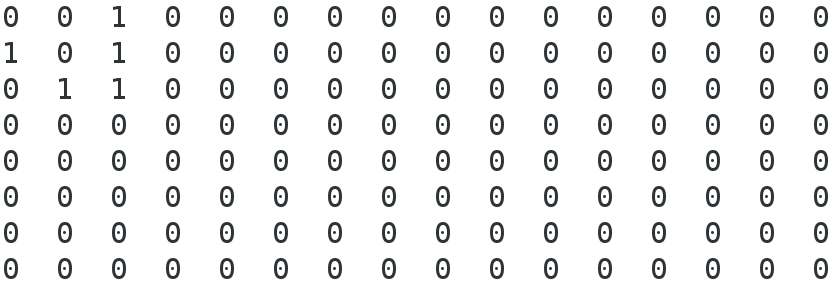
\includegraphics[width=7cm]{./images/OpenCAL/life_0000}
    \caption{Initial configuration of Game of Life, as implemented in Listing \ref{lst:cal_life}.}
    \label{fig:life_0000}
  \end{center}
\end{figure}

\begin{figure}
  \begin{center}
    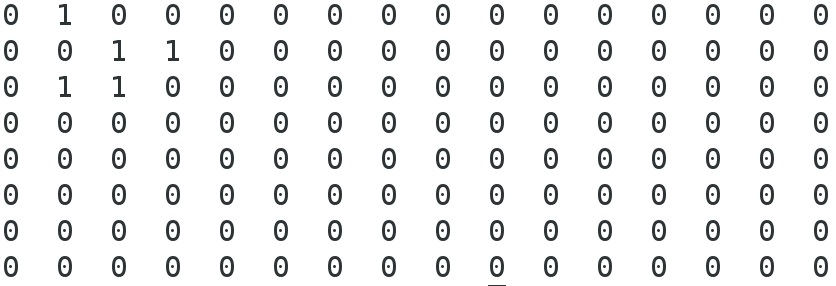
\includegraphics[width=7cm]{./images/OpenCAL/life_LAST}
    \caption{Final configuration of Game of Life (actually, just one step of computation), as implemented in Listing \ref{lst:cal_life}.}
    \label{fig:life_LAST}
  \end{center}
\end{figure}
